\documentclass[tikz,border=7pt]{standalone}
\begin{document}
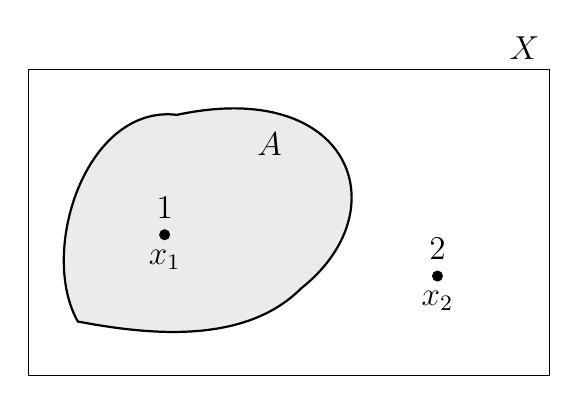
\begin{tikzpicture}[x=1.05cm,y=1.05cm,>=stealth,font=\large]
  \draw (0,0) rectangle (6.3,3.7);
  \node[above left] at (6.3,3.7) {$X$};
  \filldraw[fill=black!8,thick]
    (0.6,0.65) .. controls (0.12,1.5) and (0.7,3.28) .. (1.8,3.15)
    .. controls (3.9,3.6) and (4.5,2.0) .. (3.3,1.05)
    .. controls (2.6,0.35) and (1.4,0.5) .. cycle;
  \node at (2.92,2.8) {$A$};
  \fill (1.65,1.7) circle (2pt) (4.95,1.2) circle (2pt);
  \node[below] at (1.65,1.63) {$x_1$};
  \node[above] at (1.65,1.78) {$1$};
  \node[below] at (4.95,1.13) {$x_2$};
  \node[above] at (4.95,1.28) {$2$};
\end{tikzpicture}
\end{document}
